\documentclass[../main.tex]{subfiles}
\graphicspath{{\subfix{../media/}}}


\begin{document}

	\def\points{{2.5, 1.5, 0.9, 0.54, 0.324, 0.1944, 0.11664, 0.0699, 0.04199, 0.02519, 0.01511, 0.00906992,0.00544, 0.003265, 0.001959, 0.001175, 0.0007052, 0.0004231, 0.00025, 0.0001523}}

	\begin{figure}[h]
	    \centering
	    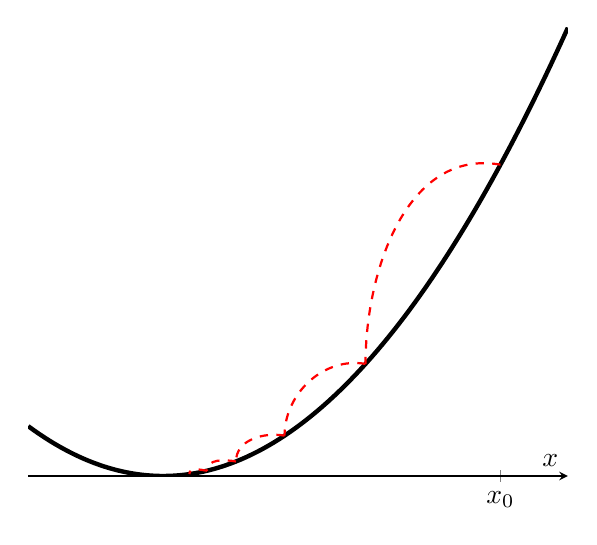
\begin{tikzpicture}
	        \begin{axis}[
	            xlabel = $x$,
	            ylabel = $f(x)$,
	            hide y axis,
	            xtick = {2.5},
	            xticklabels = {$x_0$},
	            axis lines = middle,  
	            declare function={
	                func(\x) = \x^2+1;
	            }
	        ]
	            
	            % Function
	            \addplot[ultra thick, domain=-1:3, samples=100, label={center:$f(x)$}] {func(x)};
	            
				% x/y values
				\addplot [samples at=\points, red, only marks, mark=|] {0};
				\addplot [samples at=\points, red, only marks] {func(\x)};
										
				% jumpes
			    \draw[thick, red, dashed](2.5, {func(2.5)}) to [out=170,in=90] (1.5, {func(1.5)});
			    \draw[thick, red, dashed](1.5, {func(1.5)}) to [out=170,in=90] (0.9, {func(0.9)});
			    \draw[thick, red, dashed](0.9, {func(0.9)}) to [out=170,in=90] (0.54, {func(0.54)});
			    \draw[thick, red, dashed](0.54, {func(0.54)}) to [out=170,in=90] (0.324, {func(0.324)});
			    \draw[thick, red, dashed](0.324, {func(0.324)}) to [out=170,in=90] (0.1944, {func(0.1944)});
			    				
	        \end{axis}
	    \end{tikzpicture}
	    \caption{Gradient Decent Steps}
	\end{figure}
	
\end{document}